\documentclass{article}

\usepackage[T2A]{fontenc}
\usepackage[utf8]{inputenc}
\usepackage[english, russian]{babel}

\usepackage{amssymb, amsmath, eucal, latexsym, amsthm}
\usepackage{epstopdf}
\usepackage{graphicx}
\usepackage{outlines}

\newtheorem*{theorem}{Теорема}
\newtheorem*{definition}{Определение}
\newtheorem{remark}{Замечание}

\newenvironment{psm}
	{\left( \begin{smallmatrix}}
	{\end{smallmatrix} \right) } 

\DeclareMathOperator*{\argmax}{arg\,max}

\begin{document}

\title{Теоремы о линейных операторах}

\maketitle

Рассматривается дифференциальное уравнение второго порядка с периодичной правой частью:
\begin{equation}
	u_{xx} = f(x, u), \quad f(x + L, u) = f(x, u).
\label{eq:initial}
\end{equation}
Функция $f(x, u)$ достаточно хорошая.
Периодичность правой части позволяется ввести отображение Пуанкаре $\mathcal{P}: \mathbb{R}^2 \to \mathbb{R}^2$ за период $L$, связанное с этим уравнением.
\begin{equation}
	\mathcal{P} \begin{pmatrix} u_0 \\ u_0' \end{pmatrix}
	= \begin{pmatrix} u_L \\ u_L' \end{pmatrix},
\end{equation}
где $u_L = u(L)$, $u_L' = u'(L)$, а $u(x)$ является решением уравнения \eqref{eq:initial} с начальными условиями $u(0) = u_0$, $u'(0) = u_0'$.
Отображение Пуанкаре $\mathcal{P}$, а также обратное к нему отображение $\mathcal{P}^{-1}$, могут быть определены не на всей фазовой плоскости $\mathbb{R}^2$, а лишь на некоторых её подмножествах.
Обозначим область определения отображения $\mathcal{P}$ за $\mathcal{U}_L^+$, а область определения отображения $\mathcal{P}$ за $\mathcal{U}_L^-$ соответственно.
Для дальнейшего изложения важно, чтобы совокупная область определения обоих отображений $\mathcal{U}_L = \mathcal{U}_L^+ \cap \mathcal{U}_L^-$ представляла из себя так называемое {\it островное множество}.

\begin{definition}
	Назовём {\bf островом} открытый криволинейный четырехугольник $D \subset \mathbb{R}^2$ на фазовой плоскости $(u, u')$, ограниченный двумя парами непересекающихся кривых $\alpha^{\pm}$, $\beta^{\pm}$, связанных с точками коллапса решений уравнения \eqref{eq:initial}, при этом:
	\begin{itemize}
		\item кривые $\alpha^{\pm}$ являются графиками монотонных $\gamma$-липшицевых функций $u' = h_{\pm}(u)$, а решение задачи \eqref{eq:initial} c начальными условиями $(u_0, u_0') \in \alpha^{\pm}$ коллапсирует в точке $x = -L$;
		\item кривые $\beta^{\pm}$ являются графиками монотонных $\gamma$-липшицевых функций $u = v_{\pm}(u')$, а решение задачи \eqref{eq:initial} c начальными условиями $(u_0, u_0') \in \beta^{\pm}$ коллапсирует в точке $x = +L$;
		\item если функции $h_{\pm}(u)$ являются возрастающими, тогда функции $v_{\pm}(u')$ -- убывающие, и наоборот, если функции $h_{\pm}(u)$ являются убывающими, тогда $v_{\pm}(u')$ -- возрастающие.
	\end{itemize}
\end{definition}

\begin{remark}
 	Решение задачи \eqref{eq:initial} с начальными условиями в точках пересечения кривых $\alpha^{\pm}$, $\beta^{\pm}$ коллапсирует как в точке $-L$, так и в точке $+L$.
\label{rem:alpha-beta-intersection}
\end{remark}

\begin{definition}
	Назовём множество $\mathcal{D} = \bigcup_{i = 0}^{\infty} D_i$ {\bf островным}, если оно представляет из себя счётное объединение взаимно непересекающихся островов.
\end{definition}

\begin{figure}[h]
\centering
  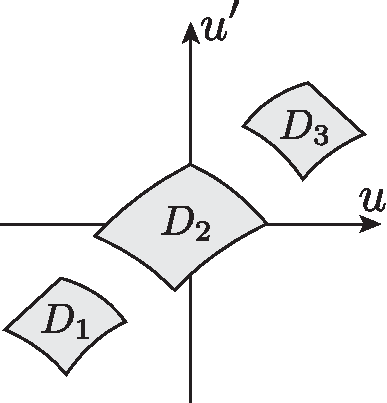
\includegraphics[scale = 0.8]{pic/set of islands}
  \caption{Пример островного множества $\mathcal{D}$ из 3-х островов.}
\label{fig:islands}
\end{figure}

Далее на островном множестве $\mathcal{D}$ введем определения v,~h~-~кривых и v,~h~-~полос соответственно.

\begin{definition}
	Пусть $D \in \mathcal{D}$ -- остров, ограниченный кривыми $\alpha^{\pm}$, $\beta^{\pm}$.
	Рассмотрим кривую $\beta$, соединяющую противолежащие стороны $\alpha^{\pm}$ острова $D$.
	Назовём такую кривую {\bf v-кривой}, если она является графиком монотонной $\gamma$-липшицевой функции $u = v(u')$, при этом тип монотонности этой функции совпадает с типом монотонности функций $u = v_{\pm}(u')$ соответствующих границам $\beta^{\pm}$ острова $D$.
	Назовём {\bf v-полосой} открытое подмножество острова $D$, ограниченное двумя \emph{v}-кривыми.
\end{definition}

\begin{definition}
	Аналогично назовём кривую $\alpha$, соединяющую границы $\beta^{\pm}$, {\bf h-кривой}, если она является графиком монотонной $\gamma$-липшицевой функции $u' = h(u)$, при этом тип её монотонности совпадает с типом монотонности границ $\alpha^{\pm}$ острова $D$.
	Назовём {\bf h-полосой} открытое подмножество острова $D$, ограниченное двумя \emph{h}-кривыми.
\end{definition}

\begin{remark}
	Сам по себе остров является предельным случаем \emph{h} и \emph{v}-полосы одновременно.
\label{rem:island}
\end{remark}



\begin{figure}[h]
\centering
  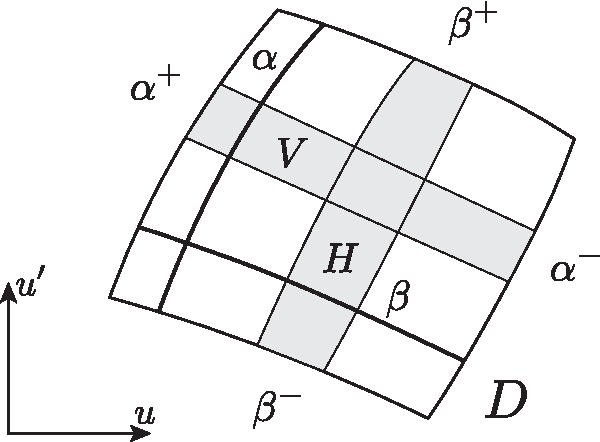
\includegraphics[scale = 0.8]{pic/curves and strips}
  \caption{Остров $D$ с границами $\alpha^+$, $\alpha^-$, $\beta^+$, $\beta^-$; h-кривая $\alpha$, v-кривая $\beta$, h-полоса $H$, v-полоса $V$.}
\label{fig:curves-and-strips}
\end{figure}

Введенные определения проиллюстрированы на рисунках \ref{fig:islands} и \ref{fig:curves-and-strips}.
Далее нам понадобится понятие ширины полос.
Ограничимся подробным изложением определений для h-полос.
Для v-полос все они записываются аналогичным образом.

Пусть h-полоса $H$ внутри острова $D$ ограничена кривыми $\alpha^+$, $\alpha^-$.
Рассмотрим графики этих кривых как функции от $u$; $\alpha^+$: $u' = h_+(u)$; $\alpha^-$: $u' = h_-(u)$.
Очевидно, что в силу геометрических особенностей острова, области определения функций $h_{\pm}(u)$ не совпадают, за исключением случая, когда границы острова $\beta^{\pm}$ являются вертикальными линиями.
Области определения функций $h_+$ и $h_-$ обозначим за $\Delta^+ = [u_0^+, u_1^+]$ и $\Delta^- = [u_0^-, u_0^+]$ соответственно.
Рассмотрим $\Delta = \Delta^+ \cup \Delta^-$ и доопределим функции $h_+$, $h_-$ на всём $\Delta$ следующим образом:
\begin{equation}
	\widetilde{h}_{\pm}(u) = \begin{cases}
		h_{\pm}(u_0^{\pm}) & u < u_0^{\pm}; \\
		h_{\pm}(u) & u \in \Delta^{\pm}; \\
		h_{\pm}(u_1^{\pm}) & u > u_1^{\pm}.
	\end{cases}
\end{equation}

В силу того, что функции $h_+$ и $h_-$ являются $\gamma$-липшицевыми на $\Delta^+$ и $\Delta^-$ соответственно, доопределённые функции $\widetilde{h}_+$ и $\widetilde{h}_-$ являются $\gamma$-липшицевыми на всём $\Delta$.
Полученные кривые обозначим за $\widetilde{\alpha}^+$ и $\widetilde{\alpha}^-$.

\begin{definition}
	Под {\bf шириной h-полосы}, ограниченной кривыми $\alpha^+$, $\alpha^-$, будем понимать расстояние между доопределёнными кривыми $\widetilde{\alpha}^+$, $\widetilde{\alpha}^-$ в смысле метрики пространства $\gamma$-липшицевых функций $C_{\gamma}(\Delta)$.
\end{definition}

\begin{remark}
 	Для двух h-полос $H_1$, $H_2$ верно $H_2 \subset H_1 \Rightarrow \Delta_2 \subseteq \Delta_1$.
\label{rem:h-strips}
\end{remark}

Для h-полосы $H$ с границами $\alpha^+$, $\alpha^-$ запишем выражение для её ширины:
\begin{equation}
	\rho(H) = \rho(\widetilde{\alpha}^+, \widetilde{\alpha}^-) = \max \limits_{u \in \Delta} |\widetilde{h}_+(u) - \widetilde{h}_-(u)|.
\label{eq:width-h-strip}
\end{equation}
Пусть максимум модуля разницы достигается в точке $u^*$, то есть
\begin{equation}
	u^* = \argmax \limits_{u \in \Delta} |\widetilde{h}_+(u) - \widetilde{h}_-(u)|.
\label{eq:argmax}
\end{equation}

\begin{definition}
	Будем говорить, что \emph{h}-полоса {\bf хорошо измерима}, если $u^* \in \Delta^+ \cap \Delta^-$.	
\end{definition}

\begin{remark}
	$\Delta^+ \cap \Delta^- \neq \varnothing \Rightarrow u^* \in \Delta^+ \cap \Delta^-$, то есть \emph{h}-полоса хорошо измерима, если области определения функций её границ имеют хотя бы одну общую точку. 
\end{remark}
\begin{proof}
	Данное утверждение непосредственно следует из монотонности границ h-полосы $\alpha^+$ и $\alpha^-$.
\end{proof}

\begin{remark}
	Любая \emph{h}-полоса, содержащаяся в хорошо измеримой \emph{h}-полосе, хорошо измерима.
\label{rem:well-h-strip}
\end{remark}

\begin{figure}[h]
\centering
  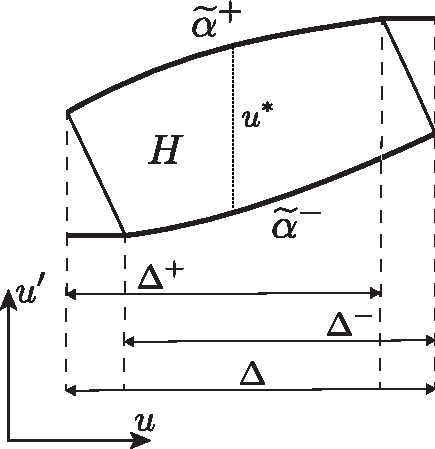
\includegraphics[scale = 0.8]{pic/width definition}
  \caption{Хорошо измеримая h-полоса $H$; доопределённые на весь интервал $\Delta$ границы $\widetilde{\alpha}^+$, $\widetilde{\alpha}^+$; точка $u^*$, в которой достигается максимум расстояния между границами, соответствует ширине полосы $H$.}
\label{fig:width-definition}
\end{figure}

Аналогичные определения вводят для v-полос подобным образом.
Введенное понятие ширины полос позволяет заменить лемму C.1 о пределе последовательности вложенных полос из оригинальной статьи \cite{ref:alfimov-avramenko-2013} полнотой пространства $\gamma$-липшицевых функций.
Понятие {\it хорошей} измеримости полос пригодится в доказательстве  нижеследующих теорем.
Оно означает, что ширину полосы можно измерить вдоль некоторой вертикальной (для h-полосы) или горизонтальной (для v-полосы) прямой, соединяющей точки с противоположных границ этой полосы.

Запишем линеаризацию отображения $\mathcal{P}$ в точке $p_0 = (u_0, u_0')$:
\begin{equation}
	\mathcal{P}(p) = \mathcal{P}_0 + D \mathcal{P}_0 (p - p_0) + o(||p - p_0||).
\label{eq:diff}
\end{equation}
Здесь $\mathcal{P}_0 = \mathcal{P}(p_0)$, а $J = D \mathcal{P}_0$ -- якобиан отображения $\mathcal{P}$ в точке $p_0$.
Линеаризация обратного отображения $\mathcal{P}^{-1}$ записывается аналогичным образом, при этом если $\mathcal{P}(p_0) = q_0$, тогда $(D \mathcal{P}_0)^{-1} = D \mathcal{P}_0^{-1}$, где $J^{-1} = D \mathcal{P}_0^{-1}$ -- якобиан обратного отображения $\mathcal{P}^{-1}$ в точке $q_0$.

Нижеследующая теорема устанавливает связь между свойствами матриц линейных операторов $D \mathcal{P}_0$, $D \mathcal{P}_0^{-1}$ и динамикой отображений $\mathcal{P}$, $\mathcal{P}^{-1}$ на фазовой плоскости.

\begin{theorem}[{\bf Об отображении h-полос}]

Пусть отображение Пуанкаре $\mathcal{P}$ и обратное к нему $\mathcal{P}^{-1}$ определены на островном множестве $\mathcal{D} = \bigcup_{i \in S} D_i$, где $S$ -- конечное множество индексов, при этом $\forall i, j \in S$ множество $V_{ij} = \mathcal{P}^{-1} D_i \cap D_j$ непусто, $\mathcal{P}$ определено на замыкании $\overline{V_{ij}}$, причём выполняется одно из двух условий:
\begin{enumerate}
	\item границы $\alpha_i^{\pm}$ острова $D_i$ являются возрастающими кривыми, а знаки элементов матрицы линейного оператора $D \mathcal{P}_0 = (a_{mn})$ имеют на всём множестве $\overline{V_{ij}}$ в точности одну из следующих конфигураций:
		\begin{center}
			(а) $\begin{psm} + & + \\ + & + \end{psm}$, \quad
			(б) $\begin{psm} - & - \\ - & - \end{psm}$, \quad
			(в) $\begin{psm} + & - \\ + & - \end{psm}$, \quad
			(г) $\begin{psm} - & + \\ - & + \end{psm}$;
		\end{center}
	\item границы $\alpha_i^{\pm}$ острова $D_i$ являются убывающими кривыми, а знаки элементов матрицы линейного оператора $D \mathcal{P}_0 = (a_{mn})$ имеют на всём множестве $\overline{V_{ij}}$ в точности одну из следующих конфигураций:
		\begin{center}
			(а) $\begin{psm} + & + \\ - & - \end{psm}$, \quad
			(б) $\begin{psm} - & - \\ + & + \end{psm}$,	\quad
			(в) $\begin{psm} + & - \\ - & + \end{psm}$, \quad
			(г) $\begin{psm} - & + \\ + & - \end{psm}$;		
		\end{center}
	\end{enumerate}
а также $\exists \mu > 1$ такое, что $\forall p_0 \in \overline{V_{ij}}$ $|a_{11}| \ge \mu$, тогда $\forall$ h-полосы $H \in \mathcal{D}$, $\forall i \in S$, $\mathcal{P} H \cap D_i = \widetilde{H}_i$ -- h-полоса, причем $\rho(\widetilde{H}_i) \le \mu \rho(H)$.

\end{theorem}

\begin{proof}
\dots
\end{proof}

Для отображения v-полос можно сформулировать полностью аналогичную теорему.

\begin{theorem}[{\bf Об отображении v-полос}]
Пусть отображение Пуанкаре $\mathcal{P}$ и обратное к нему $\mathcal{P}^{-1}$ определены на островном множестве $\mathcal{D} = \bigcup_{i \in S} D_i$, где $S$ -- конечное множество индексов, при этом $\forall i, j \in S$ множество $H_{ij} = \mathcal{P} D_i \cap D_j$ непусто, $\mathcal{P}^{-1}$ определено на замыкании $\overline{H_{ij}}$, причём выполняется одно из двух условий:
\begin{enumerate}
	\item границы $\beta_i^{\pm}$ острова $D_i$ являются возрастающими кривыми, а знаки элементов матрицы линейного оператора $D \mathcal{P}_0^{-1} = (b_{mn})$ имеют на всём множестве $\overline{H_{ij}}$ в точности одну из следующих конфигураций:
		\begin{center}
			(а) $\begin{psm} + & + \\ + & + \end{psm}$, \quad
			(б) $\begin{psm} - & - \\ - & - \end{psm}$, \quad
			(в) $\begin{psm} + & - \\ + & - \end{psm}$, \quad
			(г) $\begin{psm} - & + \\ - & + \end{psm}$;
		\end{center}
	\item границы $\beta_i^{\pm}$ острова $D_i$ являются убывающими кривыми, а знаки элементов матрицы линейного оператора $D \mathcal{P}_0^{-1} = (b_{mn})$ имеют на всём множестве $\overline{H_{ij}}$ в точности одну из следующих конфигураций:
		\begin{center}
			 (а) $\begin{psm} + & + \\ - & - \end{psm}$, \quad
			 (б) $\begin{psm} - & - \\ + & + \end{psm}$, \quad
			 (в) $\begin{psm} + & - \\ - & + \end{psm}$, \quad
			 (г) $\begin{psm} - & + \\ + & - \end{psm}$;
		\end{center}
\end{enumerate}
а также $\exists \nu > 1$ такое, что $\forall p_0 \in \overline{H_{ij}}$ $|b_{22}| \ge \nu$, тогда $\forall$ v-полосы $V \in \mathcal{D}$, $\forall i \in S$, $\mathcal{P}^{-1} V \cap D_i = \widetilde{V}_i$ -- v-полоса, причем $\rho(\widetilde{V}_i) \le \nu \rho(V)$.

\end{theorem}

\begin{proof}
	Полностью аналогично доказательству теоремы об отображении h-полос.
\end{proof}

\section*{Приложения}

\paragraph{Случай общего положения.} 

Можно просканировать фазовую плоскость с некоторым шагом и просчитать матрицы линейного оператора на множествах $\mathcal{P} D_i \cap D_j$ и $\mathcal{P}^{-1} D_i \cap D_j$, $\forall i, j$.

\paragraph{Асимптотический предел.}

Области определения внутри островов оказываются вмонтированы в асимптотические разложения.
Можно исследовать матрицы линейного оператора в асимптотическом пределе для каждой пары островов $D_i$, $D_j$.

\begin{thebibliography}{99}
\bibitem{ref:alfimov-avramenko-2013} G.~L.~Alfimov, A.~I.~Avramenko, Coding of nonlinear states for the Gross-Pitaevskii equation with periodic potential, Physica D 254 (2013) 29-45.
\end{thebibliography}

\end{document}
